\documentclass{article}
\usepackage{listings}
\usepackage{graphicx}
\usepackage{amsmath}

\lstset{
	tabsize=2
}

\title{Algorithm Design Manual Notes}
\author{Vikas Goudar}
\date{3 October, 2024}

\begin{document}
\maketitle

\newpage
\tableofcontents
\newpage

\section{Introduction to Algorithm Design}

\subsection{Insertion Sort}
Insertion sort incrementally adds an element to a sorted list and processes it
\begin{lstlisting}
insertion_sort(item s[], int n){
  int i,j; // counters 
    
  for (i = 1; i < n; ++i){
    j = i;
    while ((j > 0) && (s[j] < s[j-1])){
      swap(&s[j], &s[j-1]);
        --j;
    }
  }
}
\end{lstlisting}

\subsection{Robot Tour Optimization (TSP)}
\paragraph{Problem Statement}
There exists a robot which is used to solder points on a chip, each chip has a set of points that need to be soldered, specifically the robot is to start at a point and visit all other points and return.
Time taken is proportional to the distance travelled, and a path is to be found which minimizes time taken.

\paragraph{}
Essentially this problem, can be summarized as
\subparagraph{Input}
A set \textit{S} of \textit{n} points in the plane.
\subparagraph{Output}
Shortest cycle that visits each point in set \textit{S}

\paragraph{}
One possible solution that comes to mind (which is wrong) is to visit the node which is unvisited and closest.
However it has cases where it fails, for example refer to Figure \ref{fig:nearest_neighbor_fail_case}

\begin{figure}[h]
    \centering
    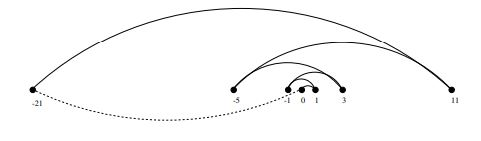
\includegraphics[width=\linewidth]{./images/robot_tour.JPG}
    \caption{Case where nearest-neighbor heurestic fails}
    \label{fig:nearest_neighbor_fail_case}
\end{figure}

\newpage

\paragraph{}
Where this algorithm fails is it doesn't know what to do in case of a tie where two nodes are equally close, and
results in paths as shown in Figure \ref{fig:nearest_neighbor_fail_case}.
\\
We try a different heurestic, one that connects closes pair of endpoints while ensuring
that their connection does prematurely end our cycle.

\paragraph{}
Initially, each vertex is treated is treated as its own seperate set, we progressively merge the sets
until one set remains.
\begin{lstlisting}
let n be the number of points in set S
for (int i = 1; i<n; ++i){
	d = inf
	for each pair of endpoints (s,t) from distinct vertex sets{
		if (dist(s, t) <= d){
			sm = s
			tm = t 
			d = dist(s, t) 
		}
	}
	connect(sm,st) -> add to same set
}
connect the last two end points remaining
\end{lstlisting}

\paragraph{}
However this algorithm also fails in certain scenarios. 
Refer to Figure \ref{fig:nearest_endpoints_heurestic_fail}

\begin{figure}[h]
    \centering
    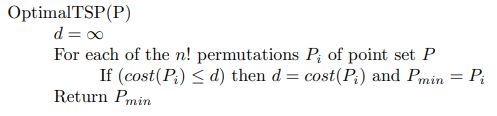
\includegraphics[width=\linewidth]{./images/robot_tour_2.JPG}
    \caption{Case where nearest-endpoints heurestic fail}
    \label{fig:nearest_endpoints_heurestic_fail}
\end{figure}

\paragraph{}
A possible fix is to try out all possible permutations and choose the optimal solution out of them.
But this is too slow.
\\
A quest to solve this problem in an efficient way is called the Travelling Salesman Problem(TSP)

\subsection{Job Scheduling}
\paragraph{}
Problem can be summarized as
\subparagraph{Input}
A Set I of n intervals
\subparagraph{Output}
Largest subset of mutually non-overlapping intervals from set I

\paragraph{}
Two possible solutions are Shortest-Job-First and Earliest-Job-First, however there exists cases
where they fail.
Refer to Figure \ref{fig:EJF_SJF_heurestic_fail}

\begin{figure}[h]
    \centering
    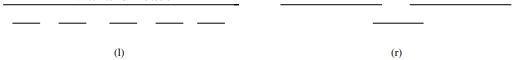
\includegraphics[width=\linewidth]{./images/job_scheduling.JPG}
    \caption{(l) earliest job first fails and (r) shortest job first fails}
    \label{fig:EJF_SJF_heurestic_fail}
\end{figure}

\paragraph{}
A brute-force method is to generate all $2^n$ subsets.
\\
Test all $2^n$ subsets of intervals and 
return the largest subset that -> consist of mutually non-overlapping intervals

\paragraph{}
However thankfully :D a better solution exists
\\
Choose the job which has earliest ending time

\begin{lstlisting}
sort jobs in ascending_order w.r.t finish_time
for (job in jobs){
	if (job.start_time >= last_end_time){
		# Process job 
		last_end_time = job.finish_time
	}
}
\end{lstlisting}

\subsection{Proof by induction/recursion}
\paragraph{}
Most of the algorithms in computer science invlove recursion/induction.
\\
There are two main steps to check if an induction/recursion algorithm is correct
\subparagraph{Base Case}
Prove that the statement $P(n)$ holds for the smallest value of n, (\textit{usually n = 0/1})
\subparagraph{Inductive Step}
Assume that $P(n)$ holds for some arbitrary number n, or every number uptil n. Then, prove that $P(n+1)$ is also true
\\
If both case hold true, the algorithm is correct for all $n \geq 0$ or any other base case.

\subparagraph{Example 1}
Prove the correctness of the following recursive algorithm foir incrementing natural numbers, $y -> y+1$

\begin{lstlisting}
Increment(y){
	if (y == 0){
		return 1
	}
	else{
		if (y mod 2){
			return 2*Increment([y/2])
		}
		else {
			return y + 1
		}
	}
}
\end{lstlisting}
\\
\textbf{Base case}: (y==0) is handled correctly.
\\
Assume the function works correctly for the general case of $F(n-1)$, now proving for general case of $F(n)$.
\\
\textbf{Even numbers}, $y+1$ is retured, so its correct
\\
\textbf{Odd numbers}, $2*Increment([y/2])$ is returned, since we our assumption holds for all cases $y \leq n-1$.

\begin{align*}
	y &= 2m + 1 \quad \text{for some integer m}\\
	2 \cdot \text{Increment} \left(\frac{2m+1}{2}\right) &= 2 \cdot \text{Increment}\left(m + \frac{1}{2}\right)\\
																											 &= 2 \cdot \text{Increment}(m)\\
																											 &= 2(m+1)\\
																											 &= 2m+2\\
																											 &= y+1
\end{align*}

\end{document}
